\chapter{Introduction}
\label{introductio}

This chapter will highlight the working environment, the project background as well as its aim.

\section{Working environment}

\subsection{University of Aalen}
The university of Aalen was founded in 1962 and by now is one of the leading university's of applied sciences in Germany. It has a focus in technical and economic research and has an approximate of 6000 students. 
The University is located in Aalen, a smaller city in the south of Germany. 

\subsection{Workshop}
The practical part of this project was carried out in my home workshop. The workshop has tools for basic metal work, wood work, a 3D-Printing as well as some tools for the development of electronics.


\section{Project background}
The mechatronic project is fixed part of the masters program "System Engineering" at Aalen University. It is supposed to cover both practical as well as theoretical work for solving a mechatronic problem.\\
In the theoretical part of the project, the problem needs to be split in smaller individual issues. In the next step, solutions for each of the issues need to be found by thoroughly analyzing the requirements of the projects.\\
In the practical part of the project, the previously discoverd issues and the solutions for it are supposed to be translated into practice. 
\begin{figure}[h!]
    \begin{center}
    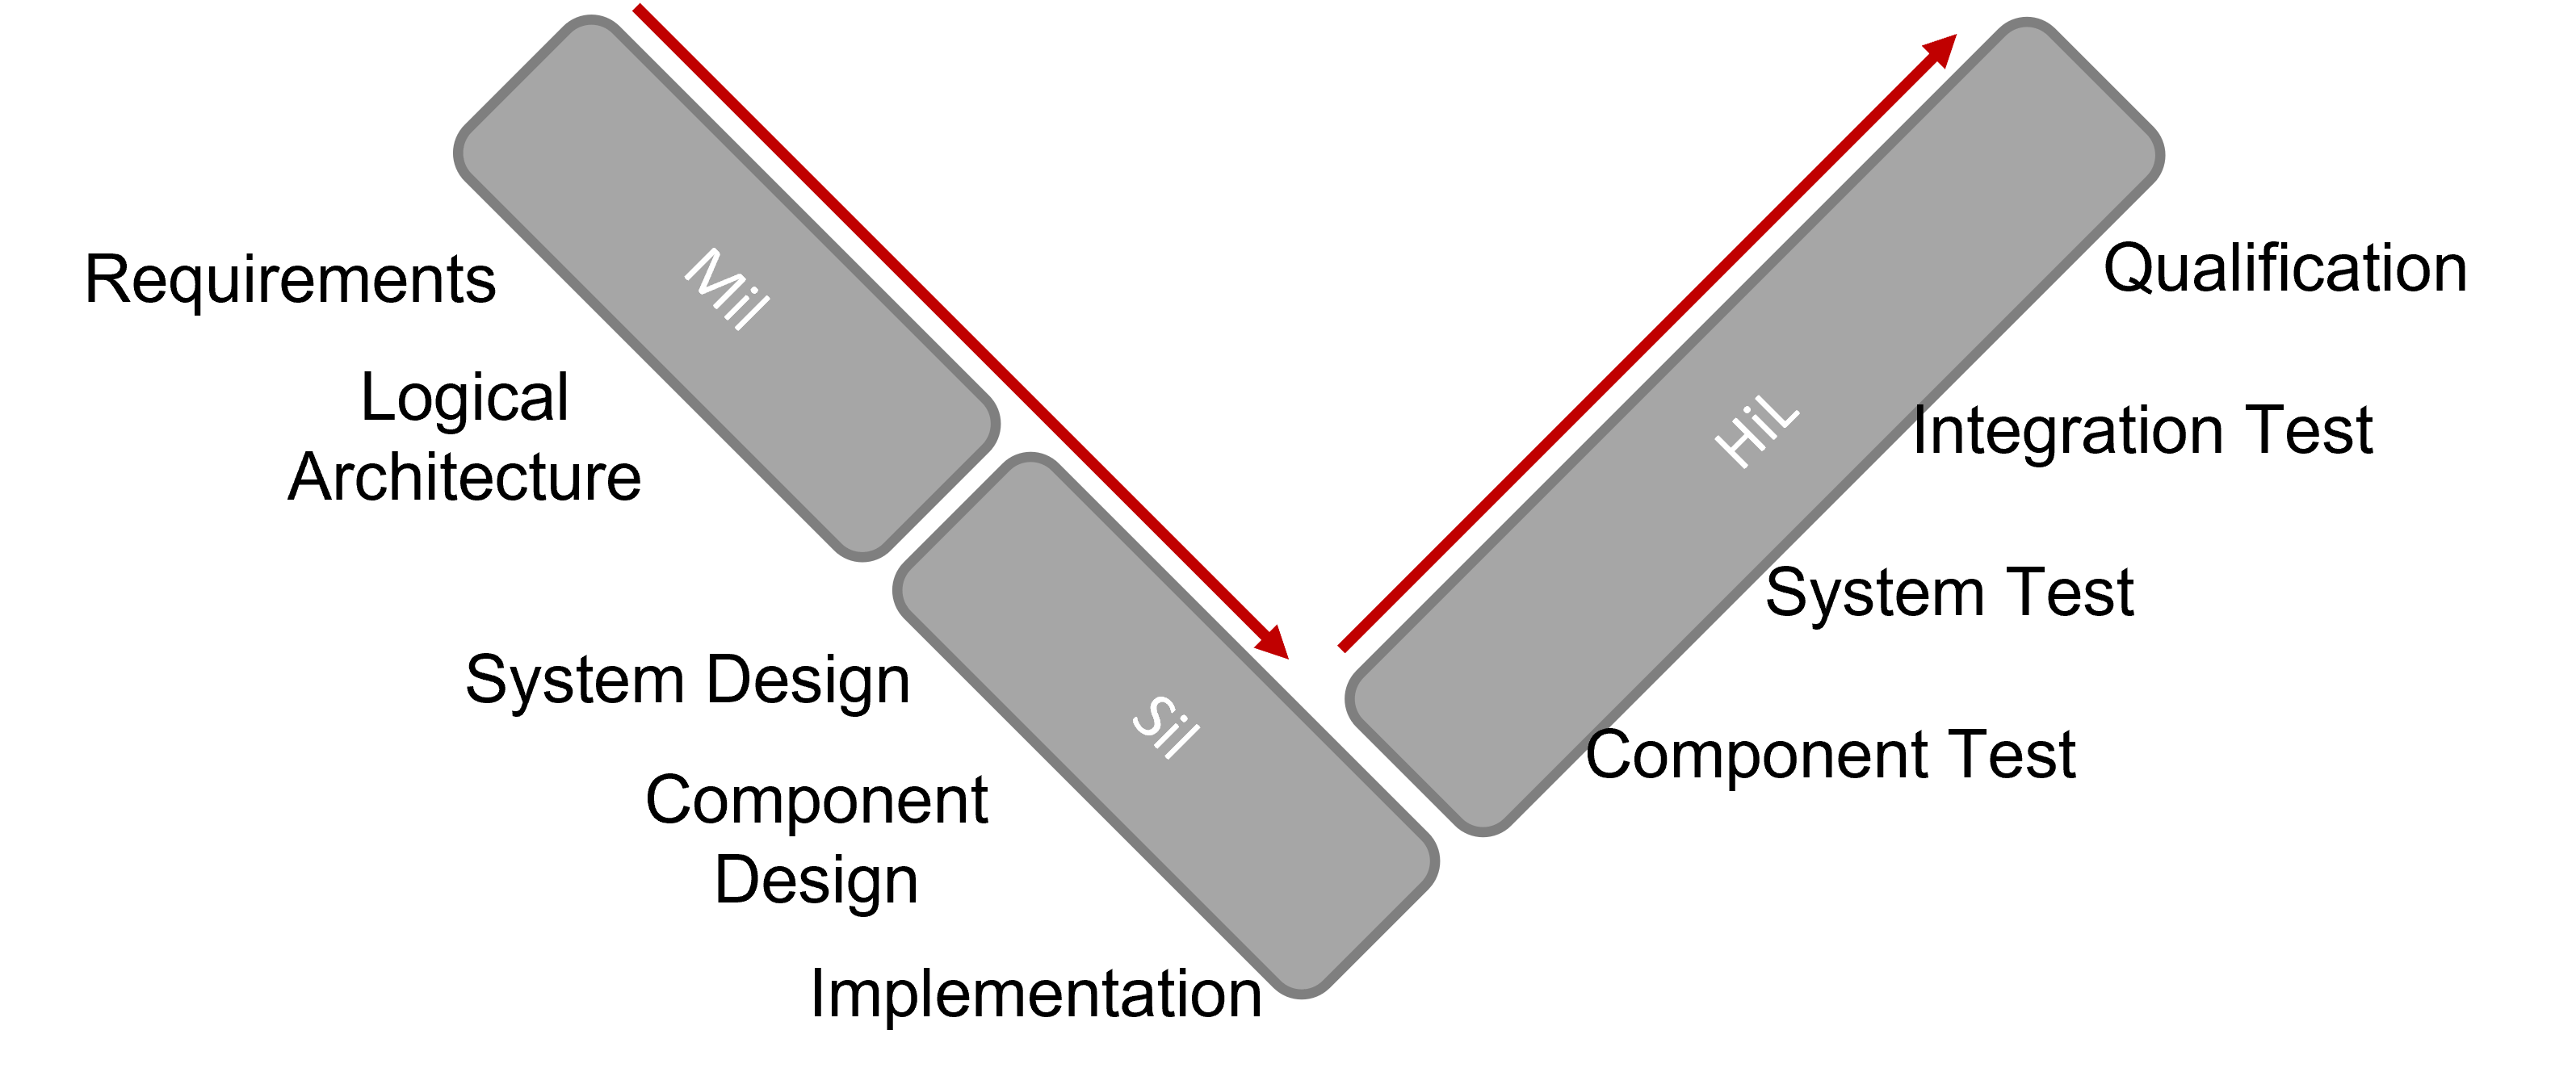
\includegraphics[width=12cm]{Pictures/VModelComplete.png}
    \caption[V-Model Complete]{V-Model}
    \label{V-Model Complete}
    \end{center}
\end{figure}

\subsection{Aim of study}


\subsection{Limitations}


